\chapter*{PERNYATAAN PENGGUNAAN AI}
\addcontentsline{toc}{chapter}{PERNYATAAN PENGGUNAAN AI}
Saya yang bertanda tangan di bawah ini menyatakan bahwa dalam penulisan dokumen Tugas Akhir ini,
saya menggunakan alat bantu kecerdasan artifisial (AI) untuk beberapa aspek tertentu di dalam proses penulisan,
seperti yang tercantum dalam tabel berikut.

\begin{table}[h]
\begin{tabular}{|p{0.5cm}| p{4cm} | p{2.5cm} | p{2.5cm} | p{3cm} @{}| }
\hline
\textbf{No.} & \textbf{Jenis} & \textbf{Alat Bantu} & \textbf{Tingkat} & \textbf{Tempat}\\
\hline
1 & Memeriksa ejaan dan tata bahasa & Claude & Sedang & Semua bab \\
\hline
2 & Pembuatan teks & Claude & Sedang & Semua bab \\
\hline
3 & Pembuatan grafik, gambar, atau ilustrasi & Claude (diagram TikZ) & Sedang & Bab III--VI \\
\hline
4 & Pencarian informasi atau referensi & Claude & Rendah & Bab II \\
\hline
5 & Penyusunan bahan diskusi & Tidak ada & Tidak ada & Tidak ada \\
\hline
6 & Penyusunan kode program & Claude Code & Sedang & Implementasi sistem \\
\hline
7 & Penyusunan formula atau perhitungan matematis & Tidak ada & Tidak ada & Tidak ada \\
\hline
8 & Penyusunan konsep desain atau algoritma & Tidak ada & Tidak ada & Tidak ada \\
\hline
9 & Penyusunan analisis data & Claude (rekap hasil uji) & Rendah & Bab VI \\
\hline
10 & Penyusunan kesimpulan atau rekomendasi & Tidak ada & Tidak ada & Tidak ada \\
\hline
\end{tabular}
\end{table}


Bandung, \today\\[0.3cm]
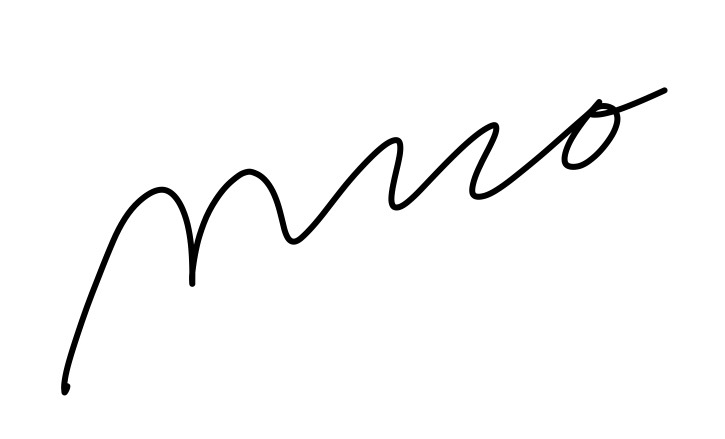
\includegraphics[height=2cm]{images/ttd.jpg}\\
\underline{Matthew Nicholas Gunawan} \\
NIM: 18222058